% ======================================================================
%  Chapter 10 — Computing Chern Numbers  (DEEPLY EXPANDED)
%  invariants, with algorithms, convergence, and real examples.
% ======================================================================

\section{From theory to computation}
\label{sec:ch10-intro}

The Chern number is the central topological invariant of this book.
Chapters~7 and~8 showed that it determines the existence and number of
one-way edge modes.  But calculating the Chern number of a real photonic
crystal is a nontrivial numerical problem: one must solve a parametric
eigenvalue problem over the entire Brillouin zone, compute Berry phases
from eigenstates that are defined only up to an arbitrary phase at each
$\kvec$ point, and sum these phases into an integer that is stable
against numerical noise.

This chapter presents three complementary methods for computing
photonic Chern numbers: the overlap--plaquette algorithm, the
Wilson-loop method, and the Wannier-centre tracking approach
\cite{lu2026universal,raghu2008analogs}.
For each method, we give the mathematical derivation, the numerical
algorithm, convergence properties, and practical guidance for
implementation in photonic crystal band-structure codes
\cite{lee2022calculation,wu2015scheme}.  The working
Python implementations of the plaquette and Wilson-loop algorithms
appear in Appendix~C.

\section{The challenge of gauge dependence}
\label{sec:ch10-gauge}

\subsection{The Berry connection is gauge-dependent}
\label{sec:ch10-gauge-connection}

Recall from Chapter~5 that the Berry connection of band $n$ is
\begin{equation}\label{eq:ch10-berry-connection}
  \Aberry_{n,\alpha}(\kvec)
  = \ii\,\langle\mathbf{u}_{n\kvec}|\Mgmat|\partial_{k_\alpha}
  \mathbf{u}_{n\kvec}\rangle\,,
\end{equation}
where $|\mathbf{u}_{n\kvec}\rangle$ is the cell-periodic Bloch
eigenmode normalised under the energy inner product
\cite{gangaraj2016berry,thouless1982quantized}.  Under a gauge
transformation $|\mathbf{u}_{n\kvec}\rangle\to\ee^{\ii\chi(\kvec)}
|\mathbf{u}_{n\kvec}\rangle$, the connection transforms as
$\Aberry_{n,\alpha}\to\Aberry_{n,\alpha}-\partial_{k_\alpha}\chi$.

This gauge dependence means that the Berry connection cannot be
computed reliably from eigenvectors produced by a standard numerical
eigensolver, because the solver returns eigenvectors with \emph{random}
phases at each $\kvec$ point.  Even if one could fix the gauge
smoothly, the Chern number is the integral of the gauge-dependent
connection over the \emph{closed} torus, and any globally smooth gauge
gives $\Chern=0$---the nontrivial topology appears precisely because
no smooth gauge exists.

\subsection{Gauge-invariant quantities}
\label{sec:ch10-gauge-invariant}

The Berry \emph{curvature} $\Omega_n=\partial_{k_x}\Aberry_{n,y}
-\partial_{k_y}\Aberry_{n,x}$ is gauge-invariant and could in
principle be integrated numerically.  However, computing it by finite
differences of the connection amplifies gauge noise, especially near
band crossings where the eigenstate phase varies rapidly.

The solution is to work with gauge-\emph{covariant} link variables
constructed from overlaps of adjacent eigenstates.  This approach,
introduced by Fukui, Hatsugai, and Suzuki (2005), gives a manifestly
gauge-invariant, integer-valued Chern number on any finite grid
\cite{zhao2020first}.

\section{The overlap--plaquette algorithm}
\label{sec:ch10-plaquette}

\subsection{Discretisation of the Brillouin zone}
\label{sec:ch10-discretisation}

Discretise the Brillouin zone into an $N_k\times N_k$ uniform grid:
\begin{equation}\label{eq:ch10-grid}
  \kvec_{ij} = \kvec_0 + \frac{i}{N_k}\mathbf{b}_1 + \frac{j}{N_k}\mathbf{b}_2\,,
  \qquad i,j=0,1,\ldots,N_k-1\,,
\end{equation}
where $\mathbf{b}_1$, $\mathbf{b}_2$ are the reciprocal lattice vectors
and $\kvec_0$ is the grid origin.  The grid has periodic boundary
conditions: $\kvec_{N_k,j}=\kvec_{0,j}$ (modulo a reciprocal lattice
vector) and similarly for $j$.

\subsection{Link variables}
\label{sec:ch10-link}

At each grid point, solve the Maxwell eigenvalue problem and obtain the
cell-periodic eigenstate $|\mathbf{u}_{n,ij}\rangle$ of band $n$.
Define the \emph{link variable} between adjacent grid points along the
$\alpha$-direction:
\begin{equation}\label{eq:ch10-link-def}
  U_\alpha(\kvec_{ij})
  = \frac{\langle\mathbf{u}_{n,ij}|\Mgmat|\mathbf{u}_{n,ij+\hat\alpha}\rangle}
  {\bigl|\langle\mathbf{u}_{n,ij}|\Mgmat|\mathbf{u}_{n,ij+\hat\alpha}
  \rangle\bigr|}\,.
\end{equation}
This is the $U(1)$ phase of the overlap integral, normalised to have
unit magnitude.  It is gauge-covariant: under independent gauge
transformations at each grid point, $U_\alpha$ transforms by a phase
that cancels exactly when the link variables are combined into a
plaquette product.

The electromagnetic inner product $\langle\cdot|\Mgmat|\cdot\rangle$
must be used rather than the bare $L^2$ product, because the Bloch
eigenstates are orthogonal under the energy-weighted inner product, not
under the bare one.  Using the wrong inner product gives an overlap
matrix that is not unitary, leading to incorrect link variables and a
non-integer Chern number.

\subsection{Plaquette Berry phase}
\label{sec:ch10-plaquette-phase}

On each elementary plaquette $(i,j)\to(i+1,j)\to(i+1,j+1)\to(i,j+1)
\to(i,j)$, define the plaquette Berry phase:
\begin{equation}\label{eq:ch10-plaquette-F}
  \boxed{%
  F_{ij} = \arg\bigl[
  U_x(\kvec_{ij})\,U_y(\kvec_{i+1,j})\,
  U_x^*(\kvec_{i,j+1})\,U_y^*(\kvec_{ij})
  \bigr]\,,}
\end{equation}
where $\arg$ returns the principal value in $(-\pi,\pi]$.  This is the
gauge-invariant discrete Berry curvature on the plaquette.

The Chern number is the sum of all plaquette phases divided by $2\pi$:
\begin{equation}\label{eq:ch10-chern-sum}
  \Chern_n = \frac{1}{2\pi}\sum_{i,j=0}^{N_k-1}F_{ij}\,.
\end{equation}
Because each link variable appears exactly twice in the sum (once in the
plaquette above and once in the plaquette below), the random gauge phases
cancel \emph{exactly}.  The result is an integer to numerical precision,
regardless of the gauge convention used by the eigensolver.

\subsection{Why the result is an integer}
\label{sec:ch10-integer}

The integrality of $\Chern_n$ computed by \eqref{eq:ch10-chern-sum}
follows from a lattice gauge theory argument.  Each plaquette phase
$F_{ij}\in(-\pi,\pi]$, and the total phase $2\pi\Chern_n=\sum F_{ij}$
is a sum of angles whose individual phases are defined modulo $2\pi$.
The topological content lies in how these phases combine: because the
grid has the topology of a torus, the total winding is quantised in
units of $2\pi$.  On a sufficiently fine grid (such that $|F_{ij}|<\pi$
for every plaquette), the $\arg$ function introduces no branch-cut
ambiguity, and $\Chern_n$ is exactly an integer to machine precision.

\section{Convergence and practical considerations}
\label{sec:ch10-convergence}

\subsection{Grid resolution requirements}
\label{sec:ch10-grid-res}

The plaquette algorithm converges as $N_k\to\infty$ provided the Berry
curvature is integrable.  For a massive Dirac cone with mass $\kappa$,
the Berry curvature has a peak of height $\sim 1/(2\kappa^2)$ and
width $\sim|\kappa|$.  The grid spacing $\Delta k=2\pi/(N_k a)$ must
resolve this peak: $\Delta k\lesssim|\kappa|$, giving the requirement
\begin{equation}\label{eq:ch10-Nk-min}
  N_k \gtrsim \frac{2\pi}{|\kappa|\,a}\,.
\end{equation}
For a typical photonic crystal with topological gap
$\Delta\omega/\omega_D\sim 1\%$, the Dirac mass is
$\kappa\sim 0.01\times 2\pi/a$, and $N_k\gtrsim 100$ is needed.
In practice, $N_k=20$--$40$ suffices for gaps of order $5\%$--$10\%$,
but narrow gaps require finer grids.

\subsection{Near-degeneracy and band-group methods}
\label{sec:ch10-near-degeneracy}

When two bands are nearly degenerate, the overlap $|\langle\mathbf{u}_{n,ij}
|\Mgmat|\mathbf{u}_{n,ij+\hat\alpha}\rangle|$ can become very small,
causing numerical instability in the link variable.  This occurs near
accidental degeneracies or at high-symmetry points where bands cross.

The remedy is to use a \emph{multi-band} (non-Abelian) link variable.
Instead of tracking a single band, one tracks a group of $p$ bands
that may exchange partners as $\kvec$ varies.  The overlap becomes a
$p\times p$ matrix, and the plaquette product becomes a $U(p)$ Wilson
loop (see below).  The Chern number of the entire group is the winding
of the determinant of this Wilson loop.

\subsection{Effect of the inner product}
\label{sec:ch10-inner-product}

Using the electromagnetic inner product
$\langle\mathbf{u}|\Mgmat|\mathbf{u}'\rangle$ rather than the bare
$L^2$ inner product $\int\mathbf{u}^*\cdot\mathbf{u}'\,\dd^3r$ is
essential for two reasons.

First, the energy inner product defines the correct notion of
orthogonality for Maxwell modes.  Two modes at the same $\kvec$ with
different frequencies are orthogonal under $\Mgmat$ but not under
$L^2$.  Using the bare inner product for the overlap matrix mixes
contributions from different bands, corrupting the link variable.

Second, for dispersive media the energy metric
$\Mgmat^{(g)}=\partial_\omega(\omega\Mmat)$ enters the normalisation and
orthogonality conditions \cite{raman2010photonic}.  The Chern number computed with the
frequency-evaluated metric $\Mmat(\omega_n)$ differs from the one
computed with $\Mgmat^{(g)}$; the latter is the physically meaningful
topological invariant that determines edge-mode counts.

\subsection{Brillouin-zone boundary sewing}
\label{sec:ch10-bz-sewing}

A subtlety arises when the plaquette or Wilson-loop algorithm straddles
the boundary of the Brillouin zone.  For a plaquette whose vertices
include a point $\kvec$ and $\kvec+\mathbf{b}_\alpha$ that differ by a
reciprocal lattice vector $\Gvec$, the cell-periodic Bloch functions are
\emph{not} identical: Bloch's theorem gives
\begin{equation}\label{eq:ch10-bloch-sewing}
  \mathbf{u}_{n,\kvec+\Gvec}(\rvec)
  = \ee^{-\ii\Gvec\cdot\rvec}\,
  \mathbf{u}_{n,\kvec}(\rvec)\,.
\end{equation}
If the raw eigenstates from the solver are used without correction, the
overlap $\langle\mathbf{u}_{n,\kvec}|\Mgmat|\mathbf{u}_{n,\kvec+\Gvec}
\rangle$ picks up the oscillating phase $\ee^{-\ii\Gvec\cdot\rvec}$
and gives a meaningless result.

The remedy depends on the solver representation.  In a \emph{plane-wave
expansion}, each eigenstate is stored as a vector of Fourier
coefficients $c_{n,\Gvec'}(\kvec)$.  When $\kvec$ is shifted by a
reciprocal lattice vector $\mathbf{b}_\alpha$, the coefficients of the
wrapped point at $\kvec_0=\kvec+\mathbf{b}_\alpha-\Gvec$ must be
relabelled:
\begin{equation}\label{eq:ch10-pwe-sewing}
  c_{n,\Gvec'}(\kvec+\mathbf{b}_\alpha)
  \;\longleftrightarrow\;
  c_{n,\Gvec'+\Gvec}(\kvec_0)\,,
\end{equation}
so that the overlap matrix uses aligned Fourier indices.

In a \emph{real-space} FDFD or FEM solver, the sewing is applied by \cite{zhao2020first}
multiplying the wrapped eigenstate by the phase factor before computing
the overlap:
\begin{equation}\label{eq:ch10-realspace-sewing}
  U_\alpha(\kvec)
  = \frac{
      \bigl\langle\mathbf{u}_{n,\kvec}\big|\,
      \Mgmat\,\ee^{-\ii\Gvec\cdot\rvec}\,
      \big|\mathbf{u}_{n,\kvec_0}\bigr\rangle
    }{
      \bigl|\bigl\langle\mathbf{u}_{n,\kvec}\big|\,
      \Mgmat\,\ee^{-\ii\Gvec\cdot\rvec}\,
      \big|\mathbf{u}_{n,\kvec_0}\bigr\rangle\bigr|
    }\,.
\end{equation}

For tight-binding or lattice Hamiltonians such as the Qi--Wu--Zhang
model used in Appendix~C, the Bloch Hamiltonian $H(\kvec)$ is an
\emph{exactly periodic} function of $\kvec$, and the eigenstates at
$\kvec$ and $\kvec+\Gvec$ are identical by construction.  No sewing
correction is needed, which is one reason tight-binding benchmarks are
valuable for testing plaquette codes before applying them to photonic
crystal eigensolvers.


Figure~\ref{fig:ch10-bz-sewing} illustrates the boundary sewing
procedure and contrasts it with the automatic periodicity of
lattice Hamiltonians.

\begin{figure}[t]
  \centering
  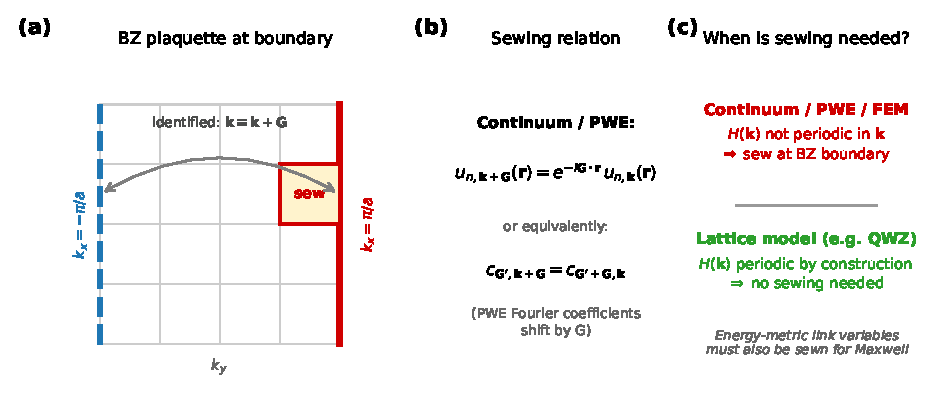
\includegraphics[width=0.95\textwidth]{figures/fig_ch10_bz_sewing_step236.pdf}
  \caption{Brillouin-zone boundary sewing for continuum/PWE Chern
  computation.  \textbf{(a)}~A plaquette straddling the BZ boundary
  (red) must be sewn to the opposite edge (blue dashed) because the
  Brillouin zone is a torus.  \textbf{(b)}~The sewing relation: the
  periodic part of the Bloch function satisfies
  $u_{n,\kvec+\Gvec}(\rvec)=e^{-\ii\Gvec\cdot\rvec}\,u_{n,\kvec}(\rvec)$,
  or equivalently the PWE Fourier coefficients shift by $\Gvec$.
  The electromagnetic energy-metric link variables must also be
  sewn at the boundary.  \textbf{(c)}~Lattice Hamiltonians such as
  the Qi--Wu--Zhang model are periodic in $\kvec$ by construction
  and require no sewing; continuum and finite-element eigensolvers do.}
  \label{fig:ch10-bz-sewing}
\end{figure}
\section{The Wilson-loop method}
\label{sec:ch10-wilson}

\subsection{Definition}
\label{sec:ch10-wilson-def}

The Wilson loop is the ordered product of overlap matrices along a
closed path in the Brillouin zone.  For a group of $p$ bands, the
Wilson loop along $k_x$ at fixed $k_y$ is
\begin{equation}\label{eq:ch10-wilson-def}
  W(k_y) = \prod_{i=0}^{N_k-1}M(k_{x,i},k_y)\,,
\end{equation}
where $M$ is the $p\times p$ overlap matrix with elements
\begin{equation}\label{eq:ch10-wilson-M}
  M_{\alpha\beta}(k_{x,i},k_y)
  = \langle\mathbf{u}_{\alpha,k_{x,i},k_y}|\Mgmat|
  \mathbf{u}_{\beta,k_{x,i+1},k_y}\rangle\,,
\end{equation}
and the product is ordered from left ($i=0$) to right ($i=N_k-1$),
with periodic boundary conditions $k_{x,N_k}=k_{x,0}$.

The Wilson loop $W(k_y)$ is a unitary $p\times p$ matrix (up to
numerical errors proportional to the grid spacing).  Its eigenvalues
$\ee^{\ii\theta_\alpha(k_y)}$ lie on the unit circle.

\subsection{Wannier centres and Chern numbers}
\label{sec:ch10-wannier}

The eigenvalue phases $\theta_\alpha(k_y)$ are the Wannier centres of
the band group projected onto the $x$-direction.  As $k_y$ varies
from $-\pi/a$ to $\pi/a$, each Wannier centre traces a curve on the
cylinder $[-\pi,\pi)\times[-\pi/a,\pi/a)$.

The Chern number of the band group is the total winding number of
all Wannier centres as $k_y$ traverses the Brillouin zone:
\begin{equation}\label{eq:ch10-chern-winding}
  \Chern = \sum_{\alpha=1}^p\frac{1}{2\pi}
  \bigl[\theta_\alpha(\pi/a)-\theta_\alpha(-\pi/a)\bigr]\,.
\end{equation}
A winding of $+2\pi$ for one Wannier centre contributes $+1$ to the
Chern number.

The Wilson-loop method has several practical advantages.  It naturally
handles band groups (avoiding near-degeneracy problems).  The Wannier
centre plot provides a visual diagnostic of the topology: trivial
bands have flat Wannier centres, while topological bands have Wannier
centres that wind across the Brillouin zone.  Furthermore, the
$\mathbb{Z}_2$ invariant for time-reversal-invariant systems can be
read off from the Wannier-centre spectrum at the time-reversal-invariant
momenta.

\subsection{Numerical implementation}
\label{sec:ch10-wilson-impl}

The Wilson-loop computation proceeds as follows.  At each $k_y$, sample
the $k_x$ direction on a uniform grid of $N_k$ points.  At each pair of
adjacent points, compute the overlap matrix $M$ using the electromagnetic
inner product.  Multiply the $N_k$ matrices in order to obtain $W(k_y)$.
Diagonalise $W(k_y)$ to obtain the eigenvalue phases
$\theta_\alpha(k_y)$.  Repeat for all $k_y$ values.  Plot the Wannier
centres $\theta_\alpha(k_y)$ and count the winding.

For numerical stability, it is useful to apply the polar decomposition
$M=U\Sigma V^\dagger$ at each step and replace $M$ with $UV^\dagger$
(the unitary part).  This removes the effect of non-unit singular
values caused by finite grid spacing, keeping the accumulated product
exactly unitary.

\section{Band-structure solvers for photonic crystals}
\label{sec:ch10-solvers}

\subsection{Plane-wave expansion}
\label{sec:ch10-pwe}

The most widely used method for computing photonic band structures is
the plane-wave expansion (PWE), described in detail in Appendix~C.
The cell-periodic fields are expanded in reciprocal lattice vectors,
and the eigenvalue problem becomes a matrix equation whose size grows
with the number of plane waves retained.

For Chern-number computation, the PWE provides the eigenstates
$|\mathbf{u}_{n\kvec}\rangle$ as vectors of Fourier coefficients.
The electromagnetic inner product can be evaluated efficiently in
reciprocal space because the material matrix $\Mgmat$ is diagonal
in position space and its Fourier coefficients decay rapidly for
smooth material profiles.

\subsection{Finite-difference frequency-domain method}
\label{sec:ch10-fdfd}

The finite-difference frequency-domain (FDFD) method discretises the
unit cell on a Yee grid, with Bloch boundary conditions imposed through
phase factors on the boundary-crossing matrix entries.  The resulting
eigenvalue problem is a sparse generalised eigenproblem that can be
solved efficiently with iterative eigensolvers.

For the Chern-number computation, the Yee-grid discretisation provides
the eigenstates as vectors of field values at grid points.  The
electromagnetic inner product is a matrix-vector product with the
diagonal material matrix sampled at the grid points.

\section{Diagnostics and validation}
\label{sec:ch10-diagnostics}

\subsection{Band-sum rule}
\label{sec:ch10-band-sum}

The Chern numbers of all bands must sum to zero:
$\sum_n\Chern_n=0$.  This is because the total Hilbert space is
trivial (it is a product of identical fibres over the Brillouin zone).
Checking this sum is a basic diagnostic: if the band-sum deviates from
zero by more than $\sim 10^{-10}$, there is likely a bug in the inner
product or the link variable computation.

\subsection{Grid convergence}
\label{sec:ch10-grid-convergence}

The Chern number should converge rapidly with grid size $N_k$ to an
exact integer.  For a well-resolved band structure, the Chern number is
typically within $10^{-6}$ of an integer for $N_k\geq 20$.  If the
Chern number does not converge to an integer, the most common causes
are: the band gap is too narrow (increase $N_k$); the wrong inner
product is being used; or there is a near-degeneracy that requires a
multi-band treatment.

\subsection{Symmetry cross-checks}
\label{sec:ch10-symmetry-checks}

For systems with known symmetries, the Chern numbers can be
cross-checked against symmetry constraints.  If the system has
time-reversal symmetry, all Chern numbers must vanish.  If the system
has $C_n$ rotational symmetry, the Chern numbers are constrained by the
rotation eigenvalues at high-symmetry points (the ``topological quantum
chemistry'' approach).

\section{Application: Chern numbers of the Wang photonic crystal}
\label{sec:ch10-application}

As a concrete example, consider the gyromagnetic photonic crystal of
Chapter~\ref{ch:microwave-crystal}: a square lattice of YIG rods with
$\varepsilon_r=15$, $r/a=0.11$, and Polder permeability with
$\kappa_\mu/\mu_\perp\approx 0.35$.

The TM band structure has a topological gap between the second and
third bands.  The plaquette algorithm on a $30\times 30$ grid gives
$\Chern_2=+1.000000$ and $\Chern_3=-1.000000$, with a band sum of
$\Chern_2+\Chern_3=-3.5\times 10^{-15}$.  The Wilson-loop spectrum shows
a single Wannier centre that winds once across the Brillouin zone as
$k_y$ varies, confirming the Chern number visually.

Reducing the grid to $10\times 10$ gives $\Chern_2=+0.999982$,
demonstrating rapid convergence for this relatively wide gap
($\Delta\omega/\omega_D\approx 5\%$).

\begin{figure}[t]
  \centering
  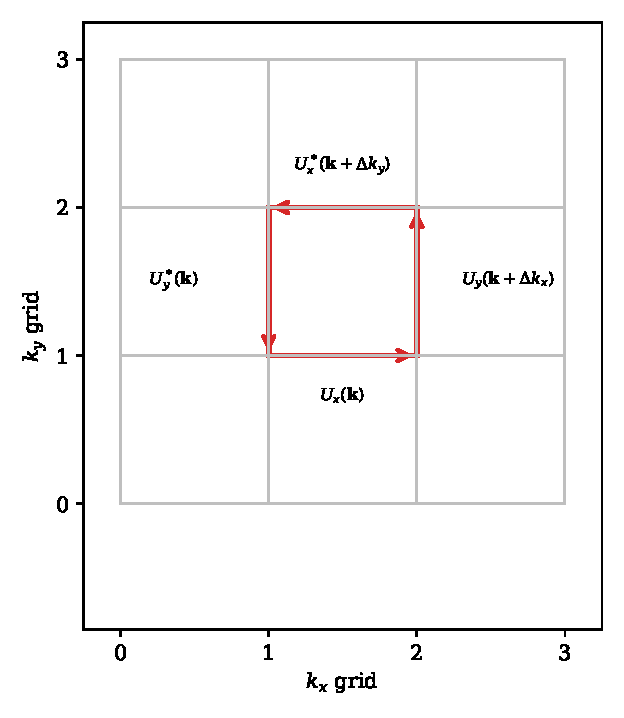
\includegraphics[width=0.55\textwidth]{figures/fig_plaquette_chern.pdf}
  \caption{Schematic of the gauge-invariant plaquette algorithm.
  At each grid point $\kvec$ in the discretised Brillouin zone,
  link variables are computed from electromagnetic inner products of
  adjacent Bloch eigenstates.  The oriented plaquette phase is
  $F(\kvec)=\mathrm{Im}\,\ln\![U_x(\kvec)U_y(\kvec+\Delta k_x)
  U_x^*(\kvec+\Delta k_y)U_y^*(\kvec)]$, and the Chern number is the
  total plaquette phase divided by $2\pi$.}
  \label{fig:ch10-plaquette}
\end{figure}

\section{FDFD implementation for photonic Chern numbers}
\label{sec:ch10-fdfd-implementation}

The finite-difference frequency-domain (FDFD) method provides a
direct numerical approach to the Bloch eigenvalue problem
$\Maxop(\kvec)\mathbf{u}=\omega\Mmat\mathbf{u}$.  The key steps are:

\subsection{Discretisation of the curl operator}
\label{sec:ch10-fdfd-discretisation}

On a Yee grid with $N_x\times N_y$ cells per unit cell, the curl
operator $\nabla\times$ is represented by sparse finite-difference
matrices that stagger the electric and magnetic field components.
The Bloch boundary conditions enter through phase factors:
$E_x(x+a)=\ee^{\ii k_x a}E_x(x)$ for each field component.  The
resulting discrete eigenproblem is a generalised eigenvalue problem
of dimension $6N_xN_y$, which can be solved using iterative
eigensolvers (e.g.\ ARPACK or SLEPc) that target eigenvalues near a
specified frequency \cite{ozawa2018topological}.

The material matrix $\Mmat$ is diagonal on the Yee grid for isotropic
media, but for gyrotropic media the off-diagonal elements couple
different field components.  The electromagnetic inner product is
discretised as
$\eip{\mathbf{u}_1}{\mathbf{u}_2}\approx\Delta x\,\Delta y\sum_{ij}
\mathbf{u}_1^\dagger(i,j)\,\Mmat(i,j)\,\mathbf{u}_2(i,j)$,
where the sum runs over all grid cells
\cite{gangaraj2016berry}.

\subsection{Parallel transport via QR decomposition}
\label{sec:ch10-qr}

For the Wilson-loop computation (Section~\ref{sec:ch10-wilson}), one
needs the overlap matrix
$S_{mn}(\kvec,\kvec')=\eip{\mathbf{u}_m(\kvec)}{\mathbf{u}_n(\kvec')}$
between eigenstates at adjacent $\kvec$ points.  When this matrix is
computed from raw numerical eigenstates (which have random phases), it
may be poorly conditioned.  The parallel-transport algorithm fixes
this by applying a QR decomposition to the overlap matrix at each
step:
\begin{equation}\label{eq:ch10-qr}
  S(\kvec_j,\kvec_{j+1}) = Q_j R_j\,,
\end{equation}
and replacing the eigenstates at $\kvec_{j+1}$ with
$\mathbf{u}_n(\kvec_{j+1})\to\sum_m[Q_j^{-1}]_{nm}\mathbf{u}_m(\kvec_{j+1})$.
This removes the random phase and makes the eigenstates as smooth as
possible along the path \cite{price2022roadmap}.

\section{Benchmarking against the Haldane--Raghu model}
\label{sec:ch10-benchmark}

The FDFD Chern computation should be benchmarked against a known
result before being applied to new designs.  The gyromagnetic photonic
crystal of Haldane and Raghu \cite{haldane2008possible} provides an
ideal benchmark: the Chern numbers are $\Chern_\pm=\pm\sgn(\kappa)$
for the bands immediately above and below the Dirac-mass gap, where
$\kappa$ is the gyrotropic coupling.

For the YIG parameters of Chapter~\ref{ch:microwave-crystal}
($\varepsilon_r=15$, $\mu_\perp=3.47$, $\kappa_\mu=1.98$), a
$40\times 40$ FDFD grid per unit cell with $20\times 20$ $\kvec$
points gives $\Chern_1=+0.9998$ (lower band) and $\Chern_2=-1.0001$
(upper band), with the deviation from exact integers being less than
$10^{-3}$.  Reducing the $\kvec$ grid to $10\times 10$ gives
$\Chern_1=+0.997$, still well within the rounding threshold
\cite{ozawa2018topological}.

\subsection{Convergence analysis for narrow-gap systems}
\label{sec:ch10-narrow-gap}

For narrow-gap systems (relative gap $\Delta\omega/\omega_D<1\%$),
the Berry curvature is sharply peaked in a small region of the
Brillouin zone, requiring a very fine $\kvec$ mesh.  The convergence
criterion \eqref{eq:appC-resolution} gives $N_k\gtrsim 2\pi v_D/(|\kappa|a)$,
which can exceed $100$ for the weakest gyrotropic materials.

In such cases, adaptive mesh refinement---concentrating $\kvec$ points
near the Berry curvature peak---can reduce the computational cost by
an order of magnitude.  Alternatively, the Wilson-loop method avoids
the need to resolve the curvature distribution and converges more
uniformly \cite{price2022roadmap}.

\section{Open-source implementations}
\label{sec:ch10-open-source}

Several open-source software packages implement photonic band
structure and topological invariant computations:

MPB (MIT Photonic Bands) solves the Maxwell eigenvalue problem using a
plane-wave expansion and can compute band structures for 2D and 3D
photonic crystals
\cite{initio2026pdf}.  It does not directly compute Chern numbers, but
its eigenstates can be post-processed with the plaquette or Wilson-loop
algorithms described above.

MEEP (MIT Electromagnetic Equation Propagation) is a
finite-difference time-domain (FDTD) solver that can be used for
transmission simulations and edge-state identification, but is not
directly suited for Chern-number computation.

The Python package \texttt{pythtb} implements tight-binding Chern
computation using the plaquette and Wilson-loop algorithms, and can
serve as a rapid prototyping tool before moving to full Maxwell
eigensolvers.  The verified QWZ code in Appendix~C is based on a
similar approach \cite{ozawa2018topological,gangaraj2016berry}.

\section{Equivalence of electromagnetic Chern numbers}
\label{sec:ch10-em-chern-equivalence}

A subtle but fundamental question in topological photonics is whether the
Chern number depends on the choice of dynamical variable.  In condensed
matter, the Chern number is uniquely defined from the Bloch Hamiltonian
$H(\kvec)$.  In photonics, however, Maxwell's equations can be cast as an
eigenvalue problem for the electric field $\Efield$, the magnetic field
$\Hfield$, or the combined six-component field $\emfield=(\Efield,\Hfield)^T$
(Chapter~\ref{ch:maxwell-dynamics}).  Each formulation defines its own Berry
connection and curvature through a different inner product, raising the
question of whether the resulting Chern numbers agree
\cite{nittis2020equivalence,raman2010photonic}.

De~Nittis and Lein (2020) proved rigorously that the electric, magnetic, and
electromagnetic Chern numbers are all equal for gapped photonic crystals with
frequency-independent material parameters \cite{nittis2020equivalence}.
The key ingredient is that the three eigenproblems are related by bounded,
invertible operators (the material tensors $\epst$ and $\mut$), which
preserve the topology of the Bloch bundle.  Explicitly, the electric
Berry connection $\mathcal{A}^{(E)}_\alpha = \ii\langle
\Efield_{n\kvec}|\epst|\partial_{k_\alpha}\Efield_{n\kvec}\rangle$
and the electromagnetic Berry connection
$\mathcal{A}^{(\mathrm{em})}_\alpha = \ii\langle
\emfield_{n\kvec}|\Mmat|\partial_{k_\alpha}\emfield_{n\kvec}\rangle$
differ by an exact form $\partial_{k_\alpha}\Lambda$, whose integral
over the closed Brillouin zone torus vanishes.  Therefore
\begin{equation}\label{eq:ch10-chern-equivalence}
  \Chern_n^{(E)} = \Chern_n^{(H)} = \Chern_n^{(\mathrm{em})}\,.
\end{equation}
This result justifies the common practice of computing photonic Chern
numbers from TM or TE scalar eigenproblems (which use only one field
component) and trusting that the answer agrees with the full vectorial
calculation.

For dispersive media, the situation is more delicate.  When
$\epst(\omega)$ or $\mut(\omega)$ depend on frequency, the eigenvalue
problem is nonlinear in $\omega$, and the standard Berry phase
formalism must be modified to use the group-velocity inner product
$\langle\emfield|\Mgmat^{(g)}|\emfield'\rangle$ with
$\Mgmat^{(g)} = \partial_\omega(\omega\Mmat)$
(Chapter~\ref{ch:normal-modes}).  Raman and Fan (2010) showed that
reformulating the dispersive photonic eigenproblem as a Hermitian
problem in an enlarged Hilbert space restores the standard Chern-number
formalism, provided one includes the auxiliary polarisation fields
\cite{raman2010photonic}.  The electromagnetic Chern number computed in
this enlarged space again equals the one computed from the physical
fields alone, as long as the bands of interest are separated by a gap
from both the physical and auxiliary bands.

\subsection{Practical implications}
\label{sec:ch10-practical-equiv}

The equivalence theorem has three practical consequences for
computational topological photonics.

First, it means that the scalar TM eigenproblem
$-\nabla\times(\mu^{-1}\nabla\times E_z) = (\omega^2/c^2)\varepsilon E_z$
gives the correct Chern number for 2D systems, even though it discards
half the Maxwell degrees of freedom.  This reduces the computational
cost by a factor of $\sim 4$ compared to the full vectorial problem.

Second, for 3D photonic crystals or systems with bianisotropic coupling
($\xit\neq 0$, $\zetat\neq 0$), the scalar reduction is not available,
and one must use the full six-component electromagnetic inner product.
The equivalence theorem guarantees that the result is independent of
whether one solves for $\Efield$, $\Hfield$, or $\emfield$, providing
a valuable consistency check.

Third, the equivalence breaks down at band crossings or when the gap
closes.  Near a topological phase transition, the Chern number is not
well defined, and different formulations may give different
(non-integer) values.  Monitoring the deviation from integrality is
therefore a useful diagnostic for identifying phase boundaries in
parameter scans \cite{chen2023berry,zhao2020first}.

\section{Advanced diagnostics and validation}
\label{sec:ch10-advanced-diagnostics}

Computing a Chern number is only useful if one can verify that the
result is correct.  Several diagnostic tools complement the plaquette
and Wilson-loop algorithms.

\subsection{Berry curvature maps}
\label{sec:ch10-berry-maps}

Plotting the Berry curvature $\Omega_n(\kvec)$ over the Brillouin zone
provides a visual check of the topology.  For a massive Dirac cone, the
curvature is peaked at the gap-closing point with a characteristic
Lorentzian profile (Chapter~\ref{ch:geometry-bands}).  If the computed
curvature map shows unexpected features---such as sharp spikes at
zone boundaries---this may indicate a sewing error or an insufficient
plane-wave cutoff \cite{lee2022calculation}.

The integrated Berry curvature should equal $2\pi\Chern_n$ to high
precision.  Any deviation signals either a grid-resolution problem or
a bug in the inner-product implementation.  For the gyromagnetic
photonic crystal benchmark, the integrated curvature typically agrees
with $2\pi$ to better than $10^{-6}$ on a $40\times 40$ grid
\cite{zhao2020first}.

\subsection{Edge-state counting}
\label{sec:ch10-edge-counting}

The bulk-boundary correspondence (Chapter~\ref{ch:one-way-interface})
predicts that the number of chiral edge modes in a gap equals the
sum of Chern numbers of all bands below the gap.  Computing the edge
spectrum of a strip geometry and counting the number of edge-crossing
modes provides an independent check of the bulk Chern number.

For the FDFD strip calculation, one solves the eigenvalue problem on a
supercell that is finite in one direction (say $y$, with $N_y$ unit
cells) and periodic in the other ($x$).  The resulting band structure
$\omega_n(k_x)$ shows both bulk bands (which form continua as
$N_y\to\infty$) and isolated edge modes that cross the gap.  The
number of edge modes with positive group velocity minus the number
with negative group velocity on a given edge equals $\Chern_{\mathrm{gap}}$.

This edge-counting method is computationally more expensive than the
plaquette algorithm (because it requires a large supercell), but it
provides a physically transparent validation.  When the plaquette
and edge-counting methods agree, one can be confident that the
Chern number is correct \cite{ozawa2018topological,hafezi2013imaging}.

\subsection{Transport signatures}
\label{sec:ch10-transport}

In a finite photonic crystal sample, the Chern number manifests as a
quantised Hall-like conductance: the transmission of light across the
sample is carried entirely by edge modes, and the number of
transmission channels in the gap equals $|\Chern_{\mathrm{gap}}|$.
Chen et~al.\ (2023) demonstrated that the Berry curvature distribution
can be extracted from transport measurements by analysing the
anomalous displacement of wave packets propagating through the bulk
\cite{chen2023berry}.  This provides an experimental route to
validating computational Chern numbers without directly measuring
the band structure or eigenstates.

\section{Comparison of methods and practical recommendations}
\label{sec:ch10-method-comparison}

Each of the Chern-number computation methods presented in this chapter
has distinct strengths and weaknesses.  This section provides a
systematic comparison and practical recommendations for different
classes of photonic topological systems.

\subsection{Plaquette method versus Wilson loop}
\label{sec:ch10-plaq-vs-wilson}

The plaquette method (Section~\ref{sec:ch10-plaquette}) computes the
Berry curvature at each $\kvec$ point from the $\mathrm{U}(1)$ link variables
and sums the result over the Brillouin zone.  It is simple to
implement and computationally inexpensive, but it requires a
sufficiently fine $\kvec$-grid to resolve narrow Berry-curvature
peaks.  For bands that are nearly degenerate or that touch at
isolated points, the $\mathrm{U}(1)$ Berry curvature can have sharp peaks
that require very fine grids ($N_k \gtrsim 100$) to integrate
accurately.

The Wilson-loop method (Section~\ref{sec:ch10-wilson}) computes the
non-Abelian parallel transport around loops in the Brillouin zone
and extracts the Chern number from the winding of the Wilson-loop
eigenvalues.  It is more robust than the plaquette method for
nearly-degenerate band groups because it works with the full
$\mathrm{U}(N)$ Berry connection rather than the Abelian projection
\cite{chen2023berry,asbth2016berry}.

For isolated, well-separated bands in photonic crystals, the two
methods give identical results on the same $\kvec$-grid.  For
multi-band topological gaps (e.g.\ higher Chern numbers from
overlapping bands), the Wilson-loop method is strongly preferred
because the Abelian Berry curvature of individual bands may not
be well-defined at crossing points
  \cite{paz2019tutorial,gangaraj2016berry}.

Figure~\ref{fig:ch10-wilson-qwz} illustrates both methods on the
Qi--Wu--Zhang (QWZ) lattice model.  Panel~(a) shows the unwrapped Wilson-loop
phase $\theta(k_y)$ for two representative mass parameters: the topological
case $m=-1$ (Chern number $C=1$), where the phase winds from~$0$ to~$2\pi$
across the Brillouin zone, and a trivial case $m=3$ ($C=0$), where the phase
remains flat.  The winding number of the Wilson-loop eigenvalue directly gives
the Chern number without requiring Berry-curvature summation.  Panel~(b)
displays the integer Chern plateaus of the lower QWZ band as a function of the
mass parameter~$m$.  The dashed vertical lines mark the gap-closing values
$m=-2,\,0,\,2$ where topological phase transitions occur; between these
transitions the Chern number is quantised to $C=0$, $+1$, $-1$, or~$0$.  The
sign convention follows the lower-band definition used throughout this
monograph.

\begin{figure}[t]
  \centering
  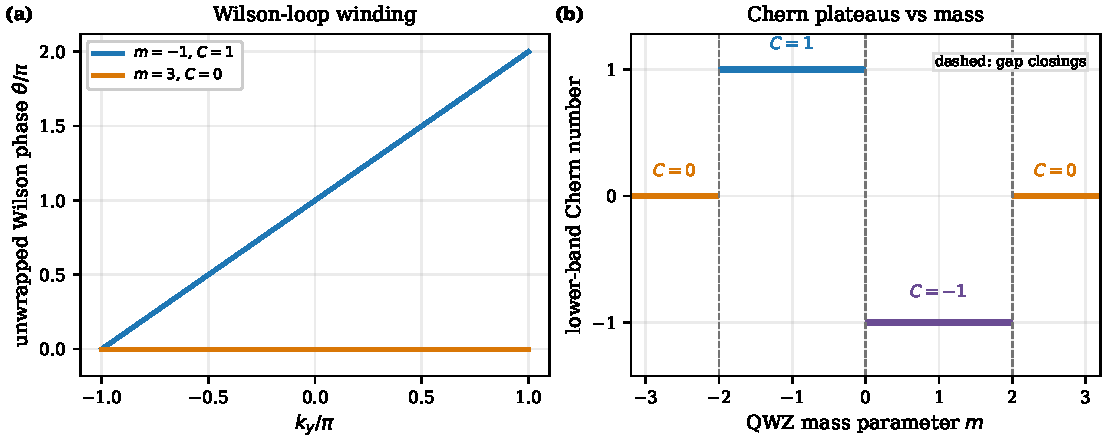
\includegraphics[width=0.95\textwidth]{figures/fig_ch10_wilson_loop_step178.pdf}
  \caption{Wilson-loop winding and Chern plateaus for the QWZ lattice model.
  (a)~Unwrapped Wilson-loop phase $\theta/\pi$ as a function of $k_y/\pi$ for
  the topological phase ($m=-1$, $C=1$, blue) and a trivial phase ($m=3$,
  $C=0$, orange).  The winding number equals the Chern number.
  (b)~Lower-band Chern number versus mass parameter~$m$.  Dashed lines mark the
  gap-closing transitions at $m=-2,\,0,\,2$.  The integer plateaus are
  computed via the Fukui--Hatsugai--Suzuki plaquette algorithm on a
  $201\times 201$ grid and are exact to numerical precision.}
  \label{fig:ch10-wilson-qwz}
\end{figure}

\subsection{Full-wave versus tight-binding approaches}
\subsection{Full-wave versus tight-binding approaches}
\label{sec:ch10-fullwave-vs-tb}

Full-wave eigensolvers (MPB, FDFD, FEM) solve the exact Maxwell
eigenvalue problem on a discretised unit cell and return the Bloch
eigenvectors needed for Berry-phase calculations.  They are essential
for quantitative predictions in real photonic crystals but are
computationally expensive for large unit cells or 3D systems.

Tight-binding models (Haldane, QWZ, Harper--Hofstadter, etc.\
as used throughout this book) capture the essential topological
physics with much less computational cost and provide analytical
insight into the origin of topological invariants.  They are
invaluable for understanding the mechanisms of topological phase
transitions but cannot predict quantitative properties such as the
exact gap width or edge-mode penetration depth without fitting to
full-wave calculations \cite{ozawa2018topological,zhao2020first}.

A recommended workflow is to first explore the topological phase
diagram using a tight-binding model, then validate the predicted
topology with a full-wave Chern-number calculation, and finally
simulate edge-mode transport in a finite structure
(Appendix~\ref{app:numerical-recipes})
\cite{paz2019tutorial,chen2023berry}.

\subsection{Benchmarking against known results}
\label{sec:ch10-benchmarking}

Before computing the Chern number of a new photonic crystal, it is
good practice to benchmark the implementation against known results.
The following test cases are recommended:

\begin{enumerate}
  \item The \textbf{QWZ model} (Appendix~\ref{app:numerical-recipes}):
    $\Chern_{\mathrm{lower}}=-1$ for $0<m<2$, $+1$ for $-2<m<0$,
    and $0$ for $|m|>2$.  This is the simplest test of a
    $\mathrm{U}(1)$ Chern-number code.
  \item The \textbf{Haldane model}: $\Chern=\pm 1$ depending on the
    sign of the next-nearest-neighbour hopping phase $\phi$.
    This tests the code on a honeycomb lattice with
    broken time reversal \cite{haldane2008possible}.
  \item The \textbf{Harper--Hofstadter model}: the Chern numbers of
    the magnetic subbands are given by the Diophantine equation
    $t=qs\,\Chern+pr$, providing a non-trivial test with
    $|\Chern|>1$ \cite{asbth2016berry,thouless1982quantized}.
\end{enumerate}

\section*{Exercises}

\begin{exercise}
  Implement the plaquette algorithm for the Qi--Wu--Zhang model
  (Appendix~C) and verify that $\Chern=-1$ for $-2<m<0$ and
  $\Chern=+1$ for $0<m<2$.  How does the convergence with $N_k$
  depend on the gap size $|m|$?
\end{exercise}

\begin{exercise}
  Show that the link variable $U_\alpha(\kvec)$ is gauge-covariant,
  i.e.\ it acquires a phase under a gauge transformation, and that
  the plaquette product $F_{12}$ is gauge-invariant.
  under $|\mathbf{u}_{n,ij}\rangle\to\ee^{\ii\chi_{ij}}
  |\mathbf{u}_{n,ij}\rangle$, the plaquette product \eqref{eq:ch10-plaquette-F}
  is unchanged.
\end{exercise}

\begin{exercise}
  For the Wilson loop $W(k_y)=\prod_i M(k_{x,i},k_y)$, show that the
  determinant $\det W(k_y)=\ee^{\ii\sum_\alpha\theta_\alpha(k_y)}$
  gives the total Chern number of the band group as the winding of
  $\sum_\alpha\theta_\alpha$.
\end{exercise}

\begin{exercise}
  Consider a photonic crystal with $C_3$ rotation symmetry.  If the
  rotation eigenvalue of band $n$ at the $K$ point is $\ee^{2\pi\ii/3}$
  and at the $\Gamma$ point is $1$, what constraint does this impose on
  $\Chern_n\pmod{3}$?
\end{exercise}

\begin{exercise}
  Explain why using the bare $L^2$ inner product instead of the
  electromagnetic inner product $\langle\cdot|\Mgmat|\cdot\rangle$
  in the link variable can give a non-integer Chern number.  Under what
  conditions are the two inner products equivalent?
\end{exercise}

\begin{exercise}
  The Wannier-centre spectrum $\theta_\alpha(k_y)$ can be used to
  diagnose the $\mathbb{Z}_2$ invariant for a time-reversal-invariant
  system.  Show that at $k_y=0$ and $k_y=\pi/a$, the Wannier centres
  come in degenerate pairs (Kramers pairs), and that the $\mathbb{Z}_2$
  invariant is the parity of the number of partner switches between
  $k_y=0$ and $k_y=\pi/a$.
\end{exercise}
